\documentclass{paper}
\usepackage{type1cm}
\usepackage{changepage}
\usepackage{caption}
\usepackage{graphicx}
\usepackage{wrapfig}

% A little bit of magic to automate numbering for the tables in Figure 1 & 2
\newcounter{magicrownumbers}[figure]
\newcommand\rownumber{\stepcounter{magicrownumbers}\arabic{magicrownumbers}.}

% Put old page numbers in the margin
\usepackage[usenames, dvipsnames]{color}
\definecolor{mygrey}{gray}{0.6}
\newcounter{oldpagecounter}
\addtocounter{oldpagecounter}{1}
\newcommand\oldpage{\stepcounter{oldpagecounter}\marginpar{\footnotesize{\textcolor{mygrey}{pg. \arabic{oldpagecounter}}}}}

\usepackage[
    backend=biber,
    style=authoryear,
    natbib=true,
    sortlocale=en_US,
    url=false, 
    doi=true,
    dashed=false,
    eprint=false,
    firstinits=true
]{biblatex}
\addbibresource{20Q.bib}

\usepackage[hidelinks, breaklinks]{hyperref}
\setlength{\parskip}{1.2ex}

\begin{document}
\title{ \mbox{You Can't Play 20 Questions with Nature and Win} \\
	 \mbox{\large Projective Comments on the Papers of This Symposium} \hspace{-0.66em}
	 \footnote{This paper appeared in W. G. Chase (ed.) (1972) Visual Information Processing, New York: Academic Press. This research was supported by Research Grant MH-07732 from the National Institutes of Health.\\ \\This version has been reformatted; the original page numbers are in the right margin.}}

\author{Allen Newell\\ \large Carnegie-Mellon University, Pittsburgh, PA}

\date{May 1973}
\maketitle
 
 
\raggedbottom
\addtolength{\topskip}{0ex plus 5ex}


I am a man who is half and half. Half of me is half distressed and half confused. Half of me is quite content and clear on where we are going. My confused and distressed half has been roused by my assignment to comment on the papers of this symposium. It is curious that it should be so. We have just listened to a sample of the best work in current experimental psychology. For instance, the beautifully symmetric RT data of Cooper and Shepard (Chapter 3) make me positively envious. It is a pleasure to watch Dave Klahr (Chapter 1) clean up the subitizing data. The demonstrations of Bransford and Johnson (Chapter 8) produce a special sort of impact. And so it goes. Furthermore, independent of the particular papers presented here, the speakers constitute a large proportion of my all-time favorite experimenters---Chase, Clark, Posner, Shepard. Not only this, but almost all of the material shown here serves to further a view of man as a processor of information, agreeing with my current 
theoretical disposition. Half of me is ecstatic.

Still, I am distressed. I can illustrate it by the way I was going to start my comments, though I could not in fact bring myself to do so. I was going to draw a line on the blackboard and, picking one of the speakers of the day at random, note on the line the time at which he got his PhD and the current time (in mid-career). Then, taking his total production of papers like those in the present symposium, I was going to compute a rate of productivity of such excellent work. Moving, finally, to the date of my chosen target's retirement, I was going to compute the total \oldpage future addition of such papers to the (putative) end of this man's scientific career. Then I was going to pose, in my role as discussant, a question: Suppose you had all those additional papers, just like those of today (except being on new aspects of the problem), \textit{where will psychology then be?} Will we have achieved a science of man adequate in power and commensurate with his complexity? And if so, how will this have happened via these papers that I have just granted you? Or will we be asking for yet another quota of papers in the next dollop of time?

Such an approach seems fairly harsh, especially to visit upon visitors. It almost made me subtitle my comments ``The Time of the Walrus'' as those of you who know their \textit{Alice Through the Looking Glass} can appreciate. The Walrus and the Carpenter invited a passel of oysters to take a pleasant walk with them---and ended up having them for lunch. Thus, I thought I'd try a different way.

\section*{Detection}

Psychology, in its current style of operation, deals with phenomena. Looking just at the local scene, we have Cooper and Shepard dealing with the phenomenon of apparent rotation, Posner (Chapter 2) dealing with the phenomenon of coding, Klahr dealing with the phenomenon of subitizing, and so on. There is, today, an amazing number of such phenomena that we deal with. The number is so large it scares me. Figure 1 gives a list of some---hardly all---that I generated in a few minutes. With each I've associated a name or two, not so much as originators (for this is not a scholarly review I am writing), but simply as an aid to identification.
\begin{table}
\begin{center}
\textsc{Phenomena}
\vspace{2ex}

\footnotesize
\begin{tabular}{l l}
\rownumber & Physical - name match difference (Posner)\\
\rownumber & Continuous rotation effect (Shepard) \\
\rownumber & Subitizing (Klahr) \\
\rownumber & Chess position perception (DeGroot) \\
\rownumber & Chunks in STM (Miller) \\
\rownumber & Recency effect in free recall (Murdock) \\
\rownumber & Instructions to forget (Bjork) \\
\rownumber & PI release (Wickens) \\
\rownumber & Linear search in sets in STM (Sternberg) \\
\rownumber & Non-improvement of STM search on success (Sternberg) \\
\rownumber & Linear search on displays (Keisser) \\
\rownumber & Non-difference of single and multiple targets in display search (Neisser) \\
\rownumber & Rapid STM loss with interpolated task (Peterson and Peterson) \\
\rownumber & Acoustic confusions in STM (Conrad) \\
\rownumber & High recognition rates for large set of pictures (Teghtsoonian and Shepard) \\
\rownumber & Visual icon (Sperling) \\ 
\rownumber & LTM hierarchy (Collins and Quillian) \\
\rownumber & LTM principle of economy (Collins and Quillian) \\
\rownumber & Successive versus paired recall in dichotic listening (Broadbent) \\
\rownumber & Click shift in linguistic expressions (Ladefoged and Broadbent) \\
\rownumber & Consistent extra delay for negation (Wason) \\
\rownumber & Saturation effect on constrained free recall (?) \\
\rownumber & Conservative probabilistic behavior (Edwards) \\
\rownumber & Clustering in free recall (Bousefield) \\
\rownumber & Constant recall per category in free recall (Tulving) \\
\rownumber & Serial position effect in free recall (?) \\
\rownumber & Backward associations Ebenholtz and Asch \\
\rownumber & Einstellung (Luchins) \\
\rownumber & Functional fixity (Dunker) \\
\rownumber & Two-state concept models (all or none learning) (Bower and Trabasso) \\
\rownumber & Concept difficulty ordering: conjunct, disjunct, cond, \ldots (Hovland) \\
\rownumber & Reversal learning (Kendlers) \\
\rownumber & von Restorff effect \\
\rownumber & Log dependency in disjunctive RT \\
\rownumber & Forward masking \\
\rownumber & Backward masking \\
\rownumber & Correlation between RT and EEG \\
\rownumber & Moon illusion (Boring) \\
\rownumber & Perceptual illusions (Mueller-Lyer, etc.) \\
\rownumber & Ambiguous figures (Necker cube) \\
\rownumber & Cyclopean perception (Julesz) \\
\rownumber & Imagery and recall (Pavio) \\
\rownumber & Constant time learning (Murdock, Bugelski) \\
\rownumber & Probability matching (Humphreys) \\
\rownumber & Transmission capacity in bits (Quastler) \\
\rownumber & Pupillary response to interest (Hess) \\
\rownumber & Stabilized images (Ditchburn) \\
\rownumber & Meaningful decay of the stabilized image (Hebb) \\
\rownumber & Categorical concepts (phonemes) (Lieberman) \\
\rownumber & Effect of marking (Clark) \\
\rownumber & Negative effect in part-whole free recall learning (Tulvlng) \\
\rownumber & Storage of semantic content over linguistic expression (Bransford) \\
\rownumber & Information addition (Anderson) \\
\rownumber & Induced chunking (Neal Johnson, Gregg and McLean) \\
\rownumber & Rehearsal \\
\rownumber & Repetitive eye scanning (Noton and Stark) \\
\rownumber & Positive effects of redundancy on learning (syntactic, semantic) \\
\rownumber & Effects of sentence transformations on recall (Miller) \\
\rownumber & Effect of irrelevant dimensions in concept learning (Restle) \\
\end{tabular}
\end{center}
\captionof{figure}{A partial list of psychological phenomena and investigators (parentheses)}
\label{fig:phenom}
\end{table}

How are these phenomena dealt with by Experimental Psychology, once brought into existence by some clever experimental discovery? Every time we find a new phenomenon---every time we find PI release, or marking, or linear search, or what-not---we produce a flurry of experiments to investigate it. We explore what it \oldpage is a function of, and the combinational variations flow from our experimental laboratories. Each of the items in Figure \ref{fig:phenom} has been the source of such a flurry. I insisted on knowing at least one ``second study'' in order to include the item in the figure; in general there are many more. Those phenomena form a veritable horn of plenty for our experimental life---the spiral of \oldpage the horn itself growing all the while it pours forth the requirements for secondary experiments. 

Do not let my description put you off. Such fecundity is a sign of vitality. We do not stay, like the medieval scholastics, forever notating and annotating the same small set of questions. The phenomena are assuredly real, the investigations surely warranted to verify their reality and confirm their nature. \oldpage

Psychology also attempts to conceptualize what it is doing, as a guide to investigating these phenomena. How do we do that? Mostly, so it seems to me, by the construction of oppositions---usually binary ones. We worry about nature versus nurture, about central versus peripheral, about serial versus parallel, and so on. To bring this point home, I give in Figure 2 a list of oppositions that have currency in psychology. These issues, I claim---about whether one or the other characterizes or explains some phenomenon---serve to drive a large part of the experimental endeavor. There are, to be sure, a few strands of theory of a different stripe, where the theory strives for some kind of quantitative explanation over a class of phenomena, parametrically expressed. I do not wish to deny these studies; neither do they dominate the current style of research enough to quiet my concern.


\begin{table}[!b]
\begin{center}
\textsc{Binary Oppositions}\\
\vspace{2ex}

\footnotesize
\begin{tabular}{l l}
\rownumber & Nature versus nurture \\
\rownumber & Peripheral versus central \\
\rownumber & Continuous versus all-or-none learning \\ 
\rownumber & Uniprocess versus duoprocess learning \\
\rownumber & Single memory versus dual memory (STM-LTM) (Melton) \\
\rownumber & Massed versus distributed practice \\
\rownumber & Serial versus parallel processing \\
\rownumber & Exhaustive versus self-terminating search \\
\rownumber & Spatial logic versus deep structure \\
\rownumber & Analog versus digital \\
\rownumber & Single code versus multiple codes \\
\rownumber & Contextual versus independent interpretation \\
\rownumber & Trace decay versus interference forgetting \\
\rownumber & Stages versus continuous development \\
\rownumber & Innate versus learned grammars (Chomsky) \\
\rownumber & Existence versus non-existence of latent learning \\
\rownumber & Existence versus non-existence of subliminal perception \\
\rownumber & Grammars versus associations for language (reality of grammar) \\
\rownumber & Conscious versus unconscious \\
\rownumber & Channels versus categorizing in auditory perception (Broadbent) \\
\rownumber & Features versus templates \\
\rownumber & Motor versus pure perception in perceptual learning \\
\rownumber & Learning on non-error trials versus learning only on error trials \\
\rownumber & Preattentive versus attentive \\
\end{tabular}
\end{center}
\captionof{figure}{A partial list of binary oppositions in psychology}
\label{oppofig}
\end{table}



I stand by my assertion that the two constructs that drive our current experimental style are (1) at a low level, the discovery and empirical exploration of phenomena such as are shown in Figure \ref{fig:phenom}; and (2) at the middle level, the formulation of questions to be put to nature that center on the resolution of binary oppositions. At the high level of grand theory, we may be driven by quite general concerns: to explore development; to discover how language is used; to show that man is a processor of information; to show he is solely analyzable in terms of contingencies of reinforcement responded to. But it is through the mediation of these lower two levels that we generate our actual experiments and give our actual explanations. Indeed, psychology with its penchant for being explicit about its methodology has created special terms, such as ``orienting attitudes'' and ``pretheoretical dispositions,'' to convey the large distance that separates the highest levels of theory from the immediate decisions of day to day science.

Accept this view, then for the moment, despite the fact that psychology like all human endeavors is too diverse to be forced into such an iron maiden. Suppose that in the next thirty years we continued as we are now going. Another hundred phenomena, give or take a \oldpage few dozen , will have been discovered and explored. Another forty oppositions will have been posited and their resolution initiated. Will psychology then have come of age? Will it provide the kind of encompassing of its subject matter---the behavior of man---that we all posit as a characteristic of a mature science? And if so, how will the transformation be accomplished by this succession of phenomena and oppositions? Same question as before, just a different lead in.

As I examine the fate of our oppositions, looking at those already in existence as a guide to how they fare and shape the course of science, it seems to me that clarity is never achieved. Matters simply become \oldpage muddier and muddier as we go down through time. Thus, far from providing the rungs of a ladder by which psychology gradually climbs to clarity, this form of conceptual structure leads rather to an ever increasing pile of issues, which we weary of or become diverted from, but never really settle. 

\begin{figure} [!b]%{L}{0.5\textwidth}
\centering
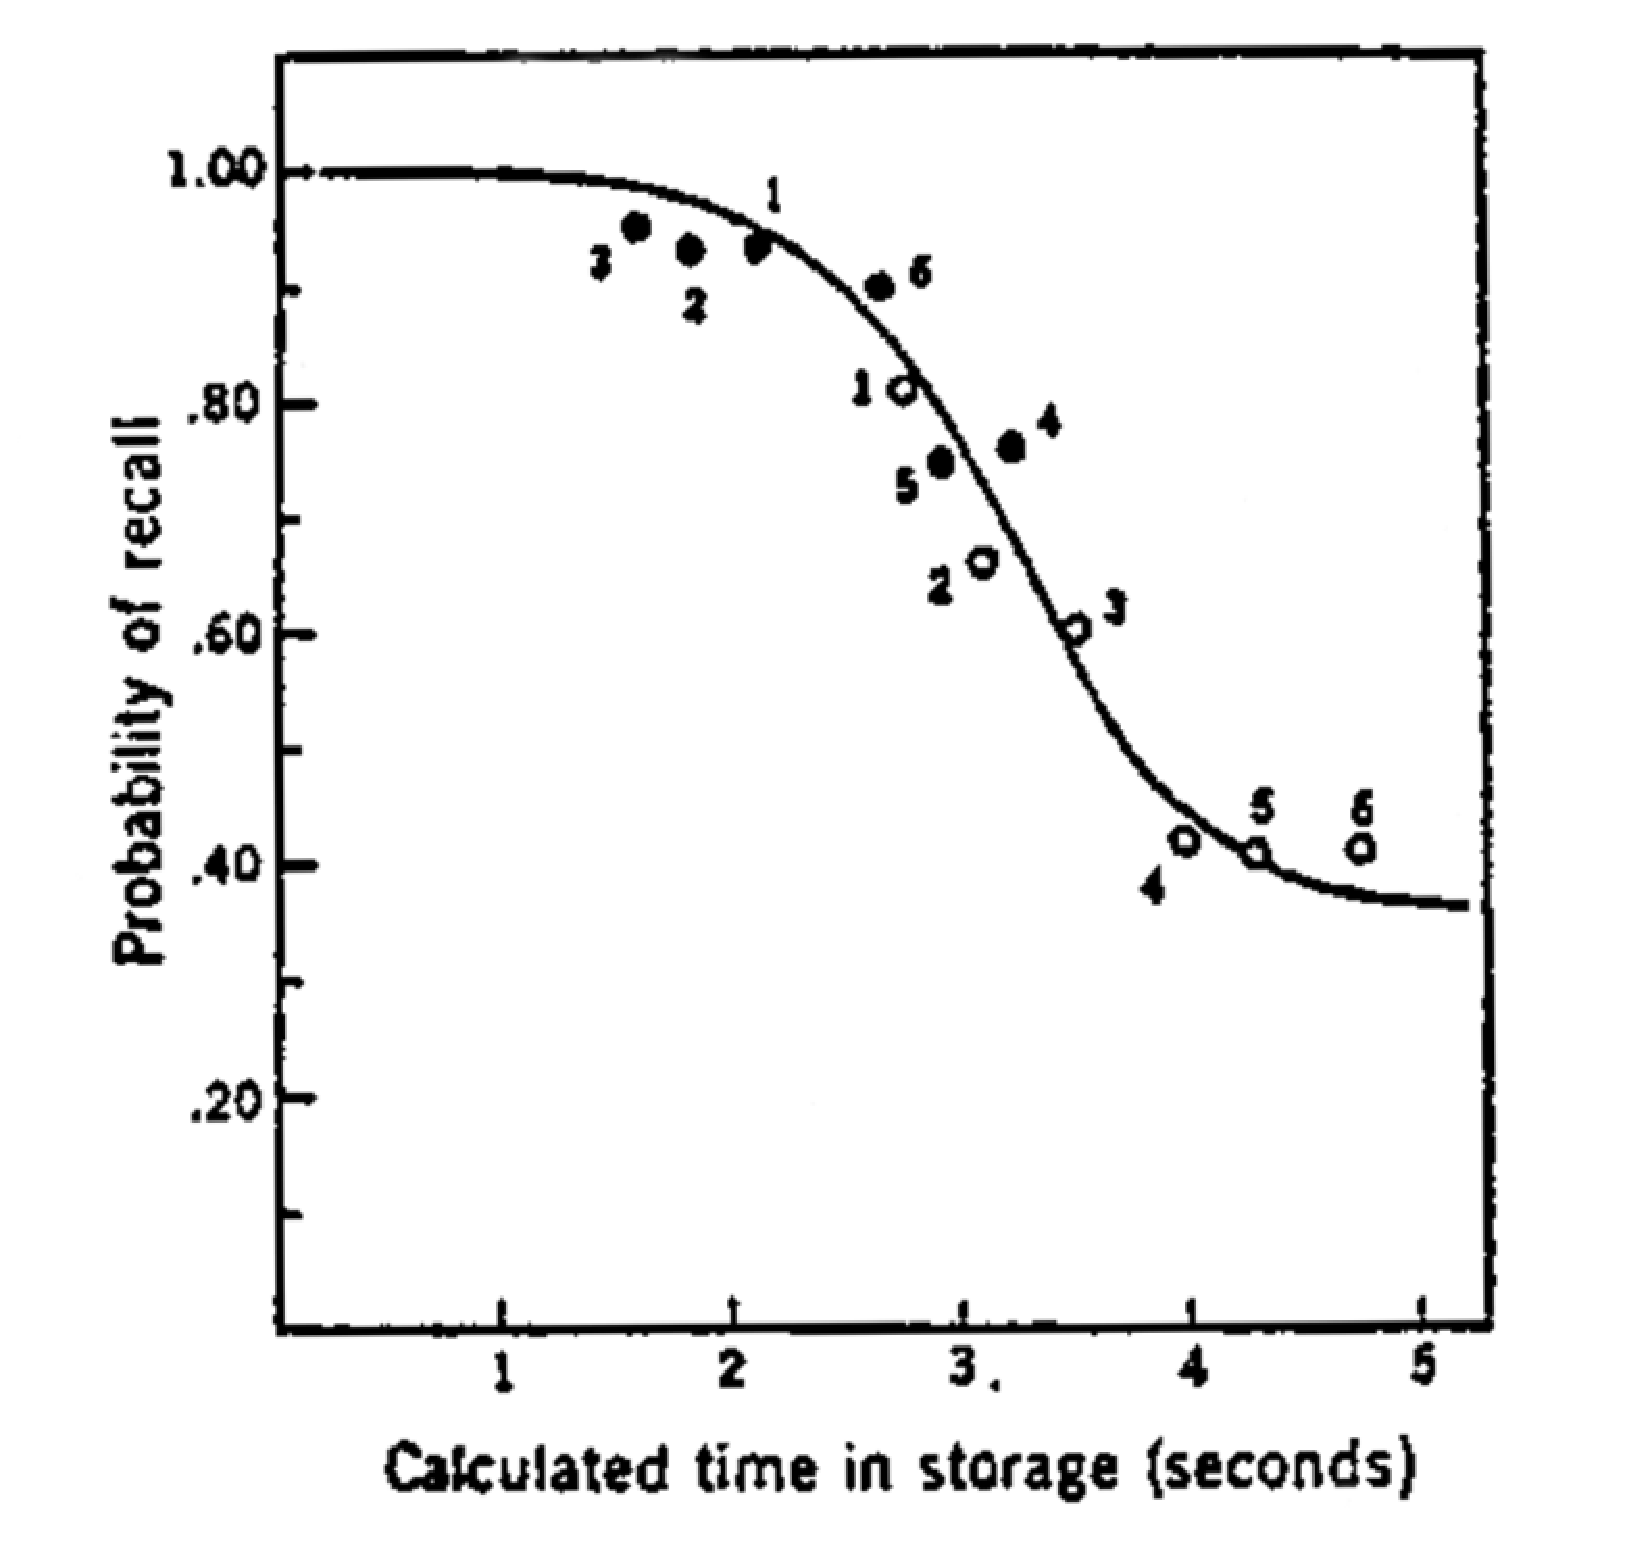
\includegraphics[width=2in]{figure3.eps}
\caption{\small Probability of recall of successive report (filled circles) and pair-by-pair report (open circles) as a function of storage time in STM \citep[after][]{WingfieldByrnes1972}}
\end{figure}

As I was preparing these comments an inadvertent illustration happened my way. The new \textit{Science} came across my desk. Sure enough, there was an article by \citet{WingfieldByrnes1972} entitled ``Decay of Information in Short Term Memory.'' They are concerned with dichotic listening. The phenomenon is that if you hear a series of stimuli simultaneously in both ears at a rapid rate there are differences in the difficulty of reporting the stimuli, depending on how they are to be grouped. If the left ear gets stimuli L1, L2, L3 and the right ear R1, R2, R3, then successive reporting (L1, L2, L3, R1, R2, R3) is easier than so-called simultaneous reporting (L1, R1, L2, R2, L3, R3). The paper reports a new explanation for the phenomenon, which is most easily understood from Figure 3 (reproduced from their article). If one considers a uniform decay curve for memory, dependent only on the length of time an item is in short term memory, then both \oldpage results follow from a detailed calculation of the lengths of time each item is in store. Thus, the grouping itself is not the operative consideration, but simply an indirect way of determining how long items must remain in memory, hence be subject to differential decay. 


The original experiments showing the phenomenon and the original explanations, in terms of time to switch a channel go back 18 years to \citet{Broadbent1958}. Furthermore, this phenomenon of simultaneous versus sequential grouping has occasioned some hundreds of papers over the intervening years, in an attempt to clarify the issues (was it channel switching or not?). Now Wingfield and Byrnes provide yet one more explanation. Regardless of the exact merits of their case---and for my purposes here I need not judge them---it can be stated with confidence that their article does not settle the issue. Theirs is just one more entry in what seems like a forever ending series of so-called clarifying experiments. With due apologies to Wingfield and Byrnes for using their work in this way (it was in fact the random occurrence noted above), it provides good evidence for the general proposition that psychological issues have difficulty even fading away.

There is, I submit, a view of the scientific endeavor that is implicit (and sometimes explicit) in the picture I have presented above. Science advances by playing twenty questions with nature. The \textit{proper} tactic is to frame a general question, hopefully binary, that can be attacked experimentally. Having settled that bits-worth, one can proceed to the next. The policy appears optimal---one never risks much, there is feedback from nature at every step, and progress is inevitable. Unfortunately, the questions never seem to be really answered, the strategy does not seem to work.

Of course I caricature. But I must get your attention. And the caricature is not so great as to be without merit.

Why do these considerations rise in me upon attempting to comment on the papers in this symposium? \oldpage First, I took as my assignment from Bill Chase to comment on them all, to the extent that I was able. To do so was probably a fateful error. Second, since I was playing the theorist, I adopted the set of trying to put them all together. \textit{Put them all together}. No doubt a compounding of the error. For not only could I not put them all together, I did not see how they themselves were putting them all together. It was exceedingly clear that each paper made a contribution. I was not exaggerating when I asserted that we have witnessed here an exceptionally fine set of experimental results and theoretical interpretations based thereon. But as I tried to put them all together, I was led back from the particular results described to a set of results that these papers referenced and used, in a qualitative sort of way. These led me back to yet other papers, many by the same group of authors and of equal merit and precision. It became less and less clear to me that all these papers were cumulating. Only the barest fraction of each prior paper found its way into the next (though fortunately there were some exceptions) , and these experiments I was considering (those today) seemed destined to play a similar role \textit{vis \`{a} vis} the future.

As I considered the issues raised (single code versus multiple code, continuous versus discrete representation, etc.) I found myself conjuring up this model of the current scientific process in psychology--- of phenomena to be explored and their explanation by essentially oppositional concepts. And I couldn't convince myself that it would add up, even in thirty more years of trying, even if one had another 300 papers of similar, excellent ilk.

In opting for worrying about this larger issue, I am not trying thereby to shirk my duty as a reviewer of the particular papers under consideration. (How often have I been annoyed as someone who was to review \textit{my} paper simply took it as the opportunity to go his own way with what \textit{he} wanted to talk about!) As an earnest of my good faith, I record herewith a sample of the direct responses generated by the specifics of the papers.\oldpage \\

\begin{adjustwidth}{2.5em}{2.5em}
\noindent \textit{To Mike Posner:} Certainly, I agree that there are multiple codes. That turns out to be almost a logical necessity. You certainly would seem to have knocked out one particular simple view. However, it would seem impossible, on the evidence that you present, to distinguish codes in the sense of the content of a representation with codes in the sense of implying separate boxes in an architectural memory structure.\\

\noindent \textit{To Lynn Cooper and Roger Shepard:} I am extraordinarily impressed by your data. However, it seems to me quite unlikely that there is a physical process of continuous rotation involved. I do not take this belief from a general bias for discrete symbolic processing (though I have that bias). Much of what is known about the visual system tells us that it is like a sampled data system---that it doesn't work continuously either in space or time \citep{HubelWiesel1962, Stark1968}. It would be surprising if (1) the visual system itself, considered as a tracking and eye-movement-controlling device, were a sampled data system, yet (2) inside that (that is, centerward from the processing of the stimulus) it became continuous again to deal with rotation. For the intuition behind the belief that rotation is to be accomplished by a continuous system is that the outside world is continuous and this should be mirrored in the internal mechanism. \\

\noindent \textit{To Bill Chase and Herb Simon:} You have clearly established that there is a phenomenon associated with chess skill, and that we have a theory now to explain how this phenomenon could arise---€”and arise in chess masters to a degree that it would not in experts or beginners. This correlational fact, however, does not yet explain why chess masters are better chess \oldpage players than beginners or experts. A natural theory is at hand given the type of theory provided; namely, a chess player will have specific actions associated with each pattern. (This is, in fact, the scheme proposed in \cite{NewellSimon1965} for guiding the tactical search, where the actions were functional move generators.) However, the theory as you present it only lays the groundwork for a theory of master level skill, and does not in any sense provide evidence for it. It requires that someone construct a program with such an arrangement and see if it plays as prescribed.\\
\end{adjustwidth}
And so it might go. But it didn't seem to me to add up to much. What I wanted was for these excellent pieces of the experimental mosaic to add up to the psychology that we all wished to foresee. They didn't, not because of any lack of excellence locally, but because most of them seemed part of a pattern of psychological activity that didn't seem able to cumulate.

\section*{Diagnosis}
Let me turn, then, from detection to diagnosis--- from assertions that we have certain difficulties that are manifest in the current pattern of our research, to an attempt to say why that is the case.

\subsection*{On Methods}
The most fundamental fact about behavior is that it is programmable. That is to say, behavior is under the control of the subject to shape in the service of his own ends. There is a sort of symbolic formula that we use in information processing psychology. To predict a subject you must know: (1) his goals; (2) the structure of the task environment; and (3) the invariant structure of his processing mechanisms. From this you \oldpage can pretty well predict what methods are available to the subject; and from the method you can predict what the subject will do. Without these things, most importantly without the method, you cannot predict what he will do. We may translate this assertion\footnote{An earlier form was the injunction to know the effective stimulus. The present formulation seems more adequate to the complexities of human behavior.}
\begin{quote}
  \textbf{First Injunction of Psychological Experimentation:} Know the method your subject is using to perform the experimental task.
\end{quote}
Uncertainty over what method the subject is using drives a substantial amount of discussion of experimental results. It is quite in evidence in the present set of papers. Klahr's discussion of why the last point in his Figure 6 (Chapter 1) is a little lower hinges on asserting the subject knows there cannot be more than five elements so he can terminate the loop early. That is, it is argued that the subject has a special method that can capitalize timewise on a bit of knowledge that we know exists in the task environment. In Cooper and Shepard's piece (Chapter 3) there is a similar concern, for instance, at what choices the subject is making at the bottom---€”whether to rotate to the left or right. In Chase and Simon's paper (Chapter 5), the entire data analysis rests, in some sense, on the method attributed to the subject for doing the tasks; and much of the side calculations (e.g., those on chunking) are done to confirm the method. Again, so it goes. In short, we are totally engaged, in psychological experimentation, in the discovery and verification of the specific methods used by the subject in doing the experimental tasks. \oldpage

The above considerations lead directly to the next assertion:
\begin{quote}
  \textbf{Second Injunction of Psychological Experimentation}: Never average
  over methods.
\end{quote}

To do so conceals, rather than reveals. You get garbage or, even worse, spurious regularity. The classic example of the failure to heed this injunction is the averaging of single-shot learning curves to yield continuous learning curves. However, we have two almost perfect examples in the present papers---perfect, not because an error was made, but because in each the authors provide data both before and after, so to speak, so one can appreciate the mis-interpretation, narrowly missed.

The first is the Cooper-Shepard data given in their Figure 5. It shows that RT is non-linear with angle of rotation. Their Figure 13 shows, however, that time is linear with angle. The explanation of the latter, as noted by Cooper and Shepard, is that it averages over all the different starting points. If they had settled for this latter data, having obtained it first, then the problem of interpretation of the non-linear curves would not have arisen---€”and we could have been led down a lovely garden path of over-simplified regularity.

The second example is from the Klahr paper. Gradually he purifies the subitizing data. At one stage (his Figure 5) we get the curve with a slope of 66 ms. However, he then separates out the instances with eye movement, leaving an additionally purified sample of response done with a single fixation and with a single subject: The slope drops to 25 ms per point in the subitizing set (his Figure 7). We are grateful for the unmixing of the methods. Can we assume to have touched bottom and that interpretation can now commence?

The point of all these remarks is that an immense amount of effort is devoted to such clarifications---that, in fact, much of the ability of the field \oldpage continually and forever to dispute and question interpretations arises from the possibility of the subject's having done the task by a not-til-then-thought-of method or by the set of subjects having adopted a mixture of methods so the regularities produced were not what they seemed. 

To put this in general terms again, our task in psychology is first to discover that structure which is fixed and invariant so that we can theoretically infer the method. Given the goal of the subject and the task environment which he faces, we can generate the (small) collection of methods that are likely to be used by him to perform the task (given his processing limits). Then, by means of careful design of the experiments or by suitable \textit{post-hoc} analysis of the subject's performance we can settle what method he did indeed use. Without such a framework within which to work, the generation of new methods, hence new explanations, for old phenomena, will go on \textit{ad nauseum}. There will be no discipline for it, as there is none now.

Let me push this branch of the diagnosis one step further. The papers of our symposium proceed by extracting for consideration a couple of mechanisms out of the totality of those required for the job. They then proceed by means of experimental technique to verify their existence, or to measure some of their properties (e.g., duration). Thus, Posner (Chapter 2) attempts (successfully, in my view) to deal with encoding of visual and auditory information, to determine whether they are the same. Sometimes more detail of a total process is presented: the flow diagrams in Cooper-Shepard, in Klahr, and in other presentations of Clark's work \citep{ClarkChase1972}. These flow diagrams serve to assert the existence of an entire set of processing stages or components and some orderings between them. 

All of the above, especially including the flow diagrams, represent major progress, both in our experimental technique and in our frameworks of interpretation. I am not here to challenge that. However \oldpage, they have in common that they leave open the total method being used. They do not operate within a frame that constrains what other methods might also be evoked to perform the same task. In short, they do not model the \textit{control} structure.

What is that, the control structure? It is best illustrated by programming languages. A language such as \textsc{Fortran} (or any other, for that matter) may be seen as a device to evoke a sequence of primitive operations, the exact sequence being conditional upon the data. The primitive operations in \textsc{Fortran} are the arithmetic operations, the given functions (sine, cosine, logarithm, etc.), the assignment of a value to a variable, the input and output operations, etc. Each of these has a name in the language (\texttt{+}, \texttt{sin}, \texttt{log}, etc.). However, just having names for the operations is not enough. Specifying the conditional sequence is also required and what does that is called the control structure. In \textsc{Fortran} it includes the syntax of algebraic expressions, which governs how the arithmetic operations are evoked, the order of statements, which implies that the operations specified by these statements are to be done in order, the syntax of the iteration statement (the \texttt{DO} statement), the format of the conditional and unconditional branch. Given the control structure, there exists a definite problem of programming to get a task done. Given only the basic operations, but not control structure, it is not possible to say what sequences of operations are or are not possible, or are possible within constraints of time and space.

Much of the new progress in the experimental analysis of the information processing of humans has eschewed attention to the control structure. The present papers of this symposium are no exception. However, my best example (my canonical one, so to speak) is the deservedly well-known paper by \cite{AtkinsonShiffrin1968} entitled: ``Human Memory: A proposed system and its control processes.'' The model of memory is there all right, and is applied to a number of tasks with quantitative precision. However, the \oldpage control structure is completely absent and is used as a \textit{deus ex machina} to concoct separate models for each task. Criticism is not directed at that justly influential piece of work. But it does illustrate well the current state of the theoretical art. As long as the control structure---the glue---is missing, so long will it be possible to suggest an indefinite sequence of alternative possibilities for how a given task was performed, hence to keep theoretical issues from becoming settled. 

\subsection*{Putting it Together}
There is a second source of our difficulties,
distinct from the one discussed above, though not unrelated to it. We never seem in the experimental literature to put the results of all the experiments together. The paper by Posner in the present symposium is an excellent example---excellent both in showing the skillful attempts we do currently make and in showing how far short this falls of really integrating the results. We do---Posner does---relate sets of experiments. But the linkage is extraordinarily loose. One picks and chooses among the qualitative summaries of a given experiment what to bring forward and juxtapose with the concerns of a present treatment.

This aspect of our current scientific style is abetted by our tendency noted at the beginning to cast the results of experiments in terms of their support or refutation of various binary oppositions. Thus, what is brought forward from an experiment is supposed to be just such qualitative summaries. Innumerable aspects of the situations are permitted to be suppressed. Thus, no way exists of knowing whether the earlier studies are in fact commensurate with whatever ones are under present scrutiny, or are in fact contradictory. Only if the contradiction is blatant, so to speak---e.g., asserting a single memory structure versus two, a long-term and a short-term memory---will the appropriate clash occur. Of course, it is not true that these other aspects are suppressed. They remain available to be \oldpage dug up by any reviewer who cares to do so, thus to keep the cycle of uncertainty and re-interpretation going.

The article of \citeauthor*{WingfieldByrnes1972} in \textit{Science}, discussed above, provides a good example of what is permissible in our present experimental style. A single result is permitted, so to speak, to challenge a rather large edifice. So loose jointed are our edifices that a divide and conquer strategy can be used. A part of the totality can be pulled out and attacked in isolation with seeming impunity.

What should be the case? A challenge to one part of a pattern of experimental results should not be permitted unless it can successfully challenge (or be shown to be consistent with) a substantial part of the total existing pattern. It is a question of where scientific responsibility lays. The warp and woof of our experimental web hangs so loose that it comes as a novel suggestion that a paper such as the Wingfield--Byrnes one is being theoretically irresponsible. 

A reaction of protest, or at least annoyance, should by now surely have set in. Am I not being harsh? How do I expect experimental work and interpretation to proceed? Isn't this the way all sciences proceed? As to the latter (since I get to give the answers, I get to select the questions), the other sciences may not have had such a slippery eel to contend with. That the same human subject can adopt many (radically different) methods for the same basic task, depending on goal, background knowledge, and minor details of payoff structure and task texture---all this---implies that the ``normal'' means of science may not suffice. As to the first question, the harshness, I restate my initial point: this is my confused and distressed half speaking. My other half is tickled pink at how fast and how far we have come in the last decade, not to speak of the last two days.

Let me stress as well that nothing in my concern implies a lessened dependence on the extraction of experimental fact or the need to develop experimental techniques. The benefits yielded to this symposium \oldpage from the chronometric analysis of reaction times, a tool that the last five years has honed to a fine edge, are immense. In fact, I really approve of all those phenomena in Figure \ref{fig:phenom}. They are examples of the kinds of experimental insights that we reap from our current investigations. I do in fact hope they double in the next ten years. My concern, to state it once more, is with how they will add up.

\section*{Prognosis}
What can be done about these concerns, assuming I have convinced you to take them seriously, at least by half? I will spend no time arguing that what is needed is to view man as an information processing system. This has been argued at length in several places (e.g., see \citet{NewellSimon1972}, for our contribution). More important, all of the papers in the present symposium are executed enough within that conceptual view to demonstrate that the lack of such a metaview is not the culprit. From this vantage point the work of Cooper and Shepard, raising as it does the possibility of continuous processing mechanisms, is as much a scientific exemplar of an information processing view as is, say, the discrete symbolic models of Chase and Simon. I will not assert that I know exactly what should be done. My distress is genuine. I am worried that our efforts, even the excellent ones I see occurring here, will not add up. Let me, however, discuss at least three possible (non-exclusive) courses of action. These might be viewed as possible paradigms within which to operate experimentally.

\subsection*{Complete Processing Models}
The first suggestion is to construct complete processing models rather than the partial ones we now do. In the present company the work of Chase and Simon fits this mold best, especially when you add to it the simulations of \cite{SimonGilmartin1973}. This theory, embodied in the simulation, actually carries out the experimental task, thus is fairly tight. \oldpage

As I noted earlier, the attempts in some of the other papers to move toward a process model by giving a flow diagram (Cooper-Shepard and Klahr\footnote{Excluding the material in Klahr's second paper
(Chapter 11).}) seem to me not to be tight enough. Too much is left unspecified and unconstrained. To make the comparison with Chase and Simon somewhat sharp, these flow diagrams are not sufficient to perform their tasks. That flow diagrams may leave something to be desired as a scheme for cumulating knowledge might be inferred from a comparison of Donald Broadbent's two books (\citeyear{Broadbent1958} and \citeyear{Broadbent1971}), both of which contain flow diagrams representing what is known (at each respective date) about short-term memory and the immediate processor. 

In one important respect, however, the Chase and Simon (and Gilmartin) work is deficient for present purposes. It does not employ a psychologically relevant model of the control processes. I argued above (and I believe) that until one has a model of the control processes (along with a model of the memories and the primitive operations) we will not be able to bring the problem of specifying subjects' methods under control.

At the moment I know of only one model of the human control processes, that of production systems \citep{NewellSimon1972, Newell1972}. These are a form of programming system that have proved useful in discussing complex cognitive tasks (such as the cryptarithmetic, logic and chess tasks treated in \citealt{NewellSimon1972}). At one level they are like any programming language, providing a way of specifying a conditional sequence of primitive operations to be applied. However, in most work on simulation programs the control structure has been treated about as casually as it is in the flow diagrams declared above to be deficient \citep[see for instance]{Johnson1964}. The production systems, by a route that need not be recounted, have become tied in with a model of the structure of memory. They \oldpage thus find themselves providing a detailed model of the control processes.

It is not my main purpose in these comments to extol the advantages of production systems. However, as noted they are the sole exemplars to my knowledge of human control processes (though they will surely not be the last). Since the notion of modeling the control and the benefits that accrue thereby in putting experimental results together is not familiar, it seems incumbent on me to provide an illustration. The attempt to do this, though it fits in this comment as a single paragraph, so to speak, is extensive enough to require an independent statement. This I have done in a companion article (Chapter 10). One should simply imagine it inserted in this essay at this point.

Let me summarize the results of that excursion \textit{vis \`{a} vis} the present argument. It is possible to construct models of the detailed control structure coupled with equally detailed assumptions about memories and elementary processes. Within such a system the question of what method the subject employs in an experimental task can be investigated in the same fashion as discovering a program in a given programming language to perform a specified task. Just as with programming, several organizations may lead to adequate performance of the task. However, each method makes definite predictions as to time and space used, providing the basis for experimental operations' to determine which method was actually operating.

There is an immense space of possible control organization and each provides a scheme within which almost any method can be programmed. Thus, the problem of determining what control system is used by the human is analogous to determining what machine language is used by a computer, given that you can never see any written code, but only the outputs of running programs. However, each control organization has different details of encoding, processing time, and memory load. They provide a basis for identifying the system experimentally if a sufficiently large and diverse set of tasks is analysed. \oldpage

\subsection*{Analyze a Complex Task}
The second experimental strategy, or paradigm, to help overcome the difficulties enumerated earlier is to accept a single complex task and do all of it. The current experimental style is to design specific small experiments to attempt to settle specific small questions---€”often as not, as I've said, dictated by the empirical exploration of a new phenomenon or by one of the polar issues. Whenever a coordinated series of experiments is created, it is usually phenomenon driven, e.g., one thinks of the sequences by Underwood and colleagues on verbal learning. The effect of this is to keep each experiment a thing-in-itself---disparate enough to guarantee the sort of loose jointed fabric I've bemoaned.

An alternative is to focus a series of experimental and theoretical studies around a single complex task, the aim being to demonstrate that one has a sufficient theory of a genuine slab of human behavior. All of the studies would be designed to fit together and add up to a total picture in detail. Such a paradigm is best described by illustration. Unfortunately, I know of no single example which successfully shows this scheme at work. I attribute this not to its difficulty but to its not really having been tried. However, let me give several partial examples.

The work of Dave Klahr provides, I believe, one example. The paper presented at this symposium is a component of a general attack on some problems of development. Initial work with a Piagetian set-inclusion task \citep{KlahrWallace1970} led to a model that depended on quantification operators. There followed a paper \citep{KlahrWallace1972} that attempted to construct a theory of quantification operators, to be used in pursuing the larger plan. The paper we heard here is a further subcomponent---the attempt to obtain some fresh data to solidify the models of quantification operators. Thus, the entire program of research is built to produce, ultimately, a complete model of the developmental set-inclusion task. I've \oldpage never explicitly asked Klahr about the strategy, but it serves my purposes to interpret it so.

A second example is a thesis done awhile ago by Donald Dansereau on mental multiplication \citep{Dansereau1969}. The goal was a theory of how people did tasks such as $17 \times 638 =\textrm{ ?}$, all in their heads. Dansereau constructed an information processing model of the process and simulated it to predict the results. That model had half a dozen or more parameters: memory transfer times, operation times, etc. The important point, for our purposes, was that he estimated all these parameters, not by fitting the simulation results to the timing data, but by conducting a series of independent micro-studies. Each of these studies was built to supply one or more parameter values to be used in the larger model. Thus, he forced a close coupling between the entire set of experimental results.

A final example, clearly mostly prospect, would be to take chess as the target super-task. We know already from existing work that the task involves forms of reasoning and search \citep{deGroot1965, NewellSimon1972, WagnerScurrah1971} and complex perceptual and memorial processes \citep[Chase \& Simon, This volume, Chapter 5]{deGroot1966}. From more general considerations we know that it also involves planning, evaluation, means-ends analysis, and redefinition of the situation, as well as several varieties of learning---short term, \textit{post-hoc} analysis, preparatory analysis, study from books, etc. Why should one not accept the task of understanding thoroughly how chess is learned and played and how this interacts with the general capabilities brought to the game? To the query of why pick chess, the response must be, Why not? Or pick another. It doesn't matter much what task is picked as long as we settle on a total complex task to force all studies into intimate relation to each other. To the point that there are lots of important mental activities not well represented by chess, the answer must be that no task is universal. What is important is to rise up a couple of levels of integration over the disaggregated scattering of tasks we now address. Concern with completeness can be saved for later iterations.\oldpage

\subsection*{One Program for Many Tasks}
The third alternative paradigm I have in mind is to stay with the diverse collection of small experimental tasks, as now, but to construct a single system to perform them all. This single system (this model of the human information processor) would have to take the instructions for each, as well as carry out the task. For it must truly be a single system in order to provide the integration that we seek.

The companion piece on productions systems (Newell, this volume, Chapter 10) in conjunction with Klahr's production system (Klahr, this volume, Chapter 11) indicates how such an endeavor might go. It is only a beginning, but it shows already a certain promise, it seems to me.

An alternative mold for such a task is to construct a single program that would take a standard intelligence test, say the \textsc{Wais} or the Stanford-Binet. This is actually an enterprise that was called for much earlier \citep{Green1964}, but only recently has anything really stirred \citep{HuntFrostLunneborg1973}.

\section*{Conclusion}
My distressed and confused half has held the ascendancy throughout this paper. I do not believe that it is just a commentator's ploy, though it emerged in the act of reviewing the papers of this symposium. It is certainly not a universal complaint I voice wherever occasion offers. Another half of my life is concerned with artificial intelligence, a part of computer science devoted to the construction of artifacts that do what mind can do---an enterprise not unrelated to the psychology of thought, though still distinct \citep{Newell1970}. There, despite the constant chorus of critics, whose universal complaint is that man and machine are of different categories, hence that progress is not possible in principle, and illusory at best, I feel that we have the ingredients of accumulation. Winograd's system (\citeyear{Winograd1972}) is a genuine advance \oldpage over the first natural language efforts. The robots do significantly better than they once did. Challengers keep showing up with programs that do all that their predecessors did and more besides.

Thus, I diagnose my concern as real. And I take seriously my call that we find some way to put it all together---€”even though this is voiced in an era when we have never been so successful experimentally and conceptually, and at a symposium where the papers exhibit so perfectly this success.

Maybe we are reaching the day of the theorist in psychology, much as it exists in other sciences such as physics. Then the task of putting things together falls to them, and experimentalists can proceed their own way. (That is not quite the way it works in physics, but no matter.) This does not seem to me our present case, but it could be. Maybe we should cooperate in working on larger experimental wholes than we now do. My positive suggestions in the prior section were proposals of how to do that. They all have in common forcing enough detail and scope to tighten the inferential web that ties our experimental studies together. This is what I think would be good for the field. Maybe we should all simply continue playing our collective game of 20 questions. Maybe all is well, as my other half assures me, and when we arrive in 1992 (the retirement date I pick might as well be my own) we will have homed in to the essential structure of the mind.

\printbibliography


\section*{Acknowledgements}
This work was supported by Public Health Service Research Grant MH-07722 from the National Institute of Mental Health.

\noindent April 2018: \href{mailto:mrkrause@gmail.com>}{Matthew Krause}  re-set a scanned copy in \LaTeX, fixed a few obvious errors and updated the citation information. The original is can be found at:\\  \url{https://pdfs.semanticscholar.org/85a0/96908670cd83cacfdede9e11f2df2dc41c9b.pdf}
\end{document}
